\documentclass[12pt,a4paper]{report}
\usepackage[utf8]{inputenc}
\usepackage[french]{babel}
\usepackage[T1]{fontenc}
\usepackage{listings}
\usepackage{xcolor}
\usepackage{amsmath}
\usepackage{graphicx}
\usepackage{float}
\usepackage{hyperref}

% Configuration des listings pour le code Draw++
\lstdefinelanguage{Draw++}{
  keywords={var, const, if, else, elif, while, for, int, float, bool, string, color,
           cursor, window, true, false, BLACK, WHITE, RED, GREEN, BLUE},
  sensitive=true,
  comment=[l]{//},
  morecomment=[s]{/*}{*/},
  morestring=[b]",
  morestring=[b]'
}

\lstset{
  language=Draw++,
  basicstyle=\ttfamily\small,
  numbers=left,
  numberstyle=\tiny,
  numbersep=5pt,
  frame=single,
  breaklines=true,
  keywordstyle=\color{blue},
  commentstyle=\color{green!60!black},
  stringstyle=\color{red},
  showstringspaces=false
}
\lstdefinestyle{customStyle}{
    basicstyle=\footnotesize\ttfamily\color{black},
    keywordstyle=\color{black},
    stringstyle=\color{black},
    commentstyle=\color{black},
    literate={é}{{\'e}}1 {è}{{\`e}}1 {à}{{\`a}}1,
    frame=single,
    breaklines=true
}




\title{Rapport de Projet : Draw++}
\author{
    Chekhab Elias \\
    Guihot Nathan \\
    Aissaoui Ahmed \\
    Zheng Lise \\
    Benmansour Firas
}
\date{\today}

\begin{document}

\maketitle
\tableofcontents

\chapter{Introduction}
Draw++ est un langage de programmation spécialement conçu pour la création graphique, visant à simplifier l'interaction avec des éléments visuels à travers un ensemble d'instructions simples et intuitives. Ce langage a été conçu pour offrir une approche accessible et directe de la programmation graphique, permettant aux utilisateurs de dessiner des formes.\\

Le projet inclut non seulement le langage de programmation proprement dit, mais aussi un environnement de développement intégré (IDE) spécialement conçu pour faciliter l'écriture, le test, et le débogage du code. L'IDE permet aux utilisateurs de visualiser immédiatement l'effet de leur code sur des graphiques à l'écran, favorisant une approche interactive et réactive de la programmation. Grâce à des fonctionnalités telles que la coloration des erreurs syntaxiques, le débogage et la gestion des erreurs, l'IDE rend l'expérience de programmation plus intuitive et accessible, même pour les débutants.

\chapter{La Syntaxe du Langage}

\section{Grammaire BNF du Langage Draw++}
Voici la grammaire formelle du langage Draw++ exprimée en notation BNF :
\begin{lstlisting}
<drawpp_program> ::= <statement_list>

<statement_list> ::= <statement> ";" | <statement> ";" <statement_list>

<statement> ::= <variable_declaration>
              | <constant_declaration>
              | <assignment>
              | <compound_assignment>
              | <if_statement>
              | <loop_statement>
              | <cursor_statement>
              | <shape_statement>
              | <comment>

<variable_declaration> ::= "var" <type> <identifier> "=" <expression>

<type> ::= "int" | "float" | "bool" | "color"

<assignment> ::= <identifier> "=" <expression>
<compound_assignment> ::= <identifier> <compound_operator> <expression>
<compound_operator> ::= "+=" | "-=" | "*=" | "/="

<if_statement> ::= "if" "(" <condition> ")" "{" <statement_list> "}"
                  [ <elif_chain> ]
                  [ "else" "{" <statement_list> "}" ]

<elif_chain> ::= "elif" "(" <condition> ")" "{" <statement_list> "}" [ <elif_chain> ]

<loop_statement> ::= <for_loop> | <while_loop>

<for_loop> ::= "for" "(" [ <variable_declaration> ] ";" <condition> ";" [ <assignment> ] ")"
               "{" <statement_list> "}"

<while_loop> ::= "while" "(" <condition> ")" "{" <statement_list> "}"

<cursor_statement> ::= <cursor_creation>
                    | <cursor_movement>
                    | <cursor_style>
                    | <cursor_visibility>

<cursor_creation> ::= "cursor" <identifier> "=" "create_cursor" "(" <expression> "," <expression> ")"

<cursor_movement> ::= <identifier> "." ( <move> | <rotate> | <position> )
<move> ::= "move" "(" <expression> ")"
<rotate> ::= "rotate" "(" <expression> ")"
<position> ::= "position" "(" <expression> "," <expression> ")"

<cursor_style> ::= <identifier> "." ( <color> | <thickness> )
<color> ::= "color" "(" <color_value> ")"
<thickness> ::= "thickness" "(" <expression> ")"

<cursor_visibility> ::= <identifier> "." "visible" "()"

<shape_statement> ::= <identifier> "." <shape_type>

<shape_type> ::= <draw_line> | <draw_rectangle> | <draw_circle> | <draw_triangle> | <draw_ellipse>

<draw_line> ::= "draw_line" "(" <expression> ")"

<draw_rectangle> ::= "draw_rectangle" "(" <expression> "," <expression> "," <bool_value> ")"

<draw_circle> ::= "draw_circle" "(" <expression> "," <bool_value> ")"

<draw_triangle> ::= "draw_triangle" "(" <expression> "," <expression> "," <bool_value> ")"

<draw_ellipse> ::= "draw_ellipse" "(" <expression> "," <expression> "," <bool_value> ")"

<color_value> ::= <predefined_color> | <custom_color>
<predefined_color> ::= "BLACK" | "WHITE" | "RED" | "GREEN" | "BLUE"
                    | "GRAY" | "LIGHT_GRAY" | "DARK_GRAY"
                    | "ORANGE" | "BROWN" | "PINK" | "CORAL" | "GOLD"
                    | "PURPLE" | "INDIGO" | "TURQUOISE" | "NAVY" | "TEAL"
                    | "FOREST_GREEN" | "SKY_BLUE" | "OLIVE" | "SALMON" | "BEIGE" | "YELLOW"
<custom_color> ::= "rgb" "(" <expression> "," <expression> "," <expression> ")"

<expression> ::= <term> | <term> <operator> <expression>
<term> ::= <identifier> | <number> | <bool_value> | <string_value>

<condition> ::= <expression> <relational_operator> <expression>
              | <bool_value>
              | <identifier>

<operator> ::= "+" | "-" | "*" | "/" | "%"
<relational_operator> ::= "<" | "<=" | ">" | ">=" | "==" | "!="

<bool_value> ::= "true" | "false"

<comment> ::= <single_line_comment> | <multi_line_comment>
<single_line_comment> ::= "//" <text> <newline>
<multi_line_comment> ::= "/*" <text> "*/"

<identifier> ::= [a-zA-Z_][a-zA-Z0-9_]*
<number> ::= [0-9]+ ( "." [0-9]+ )?
<text> ::= [^"]*
<newline> ::= "\n" | "\r\n"
\end{lstlisting}

\section{Variables Obligatoires}
Pour garantir un fonctionnement correct, chaque programme Draw++ doit définir les dimensions de la fenêtre graphique au début. Ces dimensions sont spécifiées par deux variables obligatoires :
\begin{itemize}
    \item \texttt{windowWidth} : Définit la largeur de la fenêtre.
    \item \texttt{windowHeight} : Définit la hauteur de la fenêtre.
\end{itemize}
Voici un exemple de déclaration correcte :
\begin{lstlisting}[language=Draw++]
var int windowWidth = 500;
var int windowHeight = 500;
\end{lstlisting}
Ces déclarations doivent apparaître avant toute autre instruction. Toute omission entraînera une erreur à l'exécution.

\section{Éléments de Base}

\subsection{Terminaison des Instructions}
Chaque instruction doit se terminer par un point-virgule (\texttt{;}) afin de séparer les instructions.
\begin{lstlisting}[language=Draw++]
var int x = 10;  // Déclaration d'une variable
cursor.move(100);  // Déplacement du curseur
\end{lstlisting}

\subsection{Commentaires}
Les commentaires sont ignorés à l'exécution et permettent de documenter le code :
\begin{itemize}
    \item \textbf{Commentaires sur une ligne} : Utilisez \texttt{//}.
    \item \textbf{Commentaires multi-lignes} : Utilisez \texttt{/* ... */}.
\end{itemize}
\begin{lstlisting}[language=Draw++]
// Ceci est un commentaire sur une ligne
/* Ceci est un commentaire
   multi-lignes */
\end{lstlisting}

\subsection{Délimiteurs}
Les délimiteurs structurent le code et incluent :
\begin{itemize}
    \item \texttt{\{\}} : Pour délimiter les blocs d'instructions.
    \item \texttt{()} : Pour entourer les arguments des fonctions.
\end{itemize}

\section{Types et Variables}

\subsection{Déclaration des Variables}
Les variables sont déclarées avec le mot-clé \texttt{var}, suivi de leur type, de leur nom et de leur valeur initiale.
\begin{lstlisting}[language=Draw++]
var int compteur = 0;
var float pi = 3.14159;
var color myColor = rgb(255, 0, 0);
var bool isFilled = true;
\end{lstlisting}

\section{Structures de Contrôle}

\subsection{Conditions}
Les structures conditionnelles permettent d'exécuter des blocs de code selon des conditions :
\begin{itemize}
    \item \texttt{if (<condition>) { <bloc d'instructions> }}
    \item \texttt{elif (<condition>) { <bloc d'instructions> }}
    \item \texttt{else { <bloc d'instructions> }}
\end{itemize}

\subsection{Boucles}
Draw++ prend en charge deux types de boucles principales :
\begin{itemize}
    \item \texttt{while (<condition>) { <bloc d'instructions> }}
    \item \texttt{for (<initialisation>; <condition>; <mise à jour>) { <bloc d'instructions> }}
\end{itemize}

\section{Manipulation du Curseur}
Le curseur est l'objet central pour dessiner. Il est défini avec la syntaxe suivante :
\begin{lstlisting}[language=Draw++]
cursor <identifiant> = create_cursor(<x>, <y>);
\end{lstlisting}
Les propriétés et méthodes principales du curseur incluent :
\begin{itemize}
    \item \texttt{cursor.move(distance)} : Déplace le curseur.
    \item \texttt{cursor.rotate(angle)} : Tourne le curseur.
    \item \texttt{cursor.color(<couleur>)} : Définit la couleur.
    \item \texttt{cursor.thickness(<valeur>)} : Définit l'épaisseur du trait.
    \item \texttt{cursor.visible()} : Contrôle la visibilité du curseur.
\end{itemize}
Exemple de création et utilisation du curseur :
\begin{lstlisting}[language=Draw++]
cursor c = create_cursor(0, 0);
c.color(RED);
c.move(50);
\end{lstlisting}

\section{Dessiner des Formes}
Les formes peuvent être dessinées avec les méthodes du curseur :
\begin{itemize}
    \item \texttt{cursor.draw\_line(longueur)} : Dessine une ligne.
    \item \texttt{cursor.draw\_rectangle(largeur, hauteur, rempli)} : Dessine un rectangle.
    \item \texttt{cursor.draw\_circle(rayon, rempli)} : Dessine un cercle.
    \item \texttt{cursor.draw\_triangle(base, hauteur, rempli)} : Dessine un triangle.
    \item \texttt{cursor.draw\_ellipse(largeur, hauteur, rempli)} : Dessine une ellipse.
\end{itemize}
Exemples :
\begin{lstlisting}[language=Draw++]
// Dessiner une ligne
cursor c = create_cursor(0, 0);
c.draw_line(100);

// Dessiner un rectangle rempli
c.draw_rectangle(50, 100, true);

// Dessiner un cercle non rempli
c.draw_circle(30, false);
\end{lstlisting}

\section{Couleurs et Styles}
Le curseur peut être personnalisé avec des couleurs prédéfinies ou des couleurs personnalisées. Exemple :
\begin{lstlisting}[language=Draw++]
c.color(RED);
c.thickness(3);  // Définit l'épaisseur du trait
c.color(rgb(255, 0, 0));  // Rouge personnalisé
\end{lstlisting}



\chapter{Description du traducteur}

\section{Architecture du traducteur}
Le traducteur de Draw++ est un système qui convertit le code source écrit dans le langage Draw++ en code C intermédiaire, prêt à être compilé. Ce processus de traduction s'effectue en plusieurs étapes clés, chacune ayant pour but de transformer le code dans un format plus proche de l'exécution.

\begin{enumerate}
    \item \textbf{Analyse lexicale} : Dans cette phase, le code source est décomposé en tokens, qui sont les plus petites unités syntaxiques. Par exemple, des mots-clés comme \texttt{cursor}, \texttt{var}, \texttt{if}, ainsi que les identifiants et les opérateurs, sont extraits du code source.
    \item \textbf{Analyse syntaxique} : Une fois que les tokens ont été générés, le traducteur construit un arbre syntaxique abstrait (AST). Cet arbre représente la structure logique du programme, où chaque nœud correspond à une construction du langage (par exemple, une expression, une condition, ou une affectation).
    \item \textbf{Analyse sémantique} : À ce stade, le traducteur vérifie la validité des types, la cohérence des variables, et l'intégrité du programme. Cette étape s'assure que les opérations sont effectuées sur des types compatibles (par exemple, éviter de tenter d'ajouter un entier à une chaîne de caractères).
    \item \textbf{Génération de code} : Enfin, le traducteur génère le code C intermédiaire, qui est une version optimisée et exécutable de l'AST. Ce code est ensuite prêt à être compilé par un compilateur C classique.
\end{enumerate}

\section{Processus de traduction}
Prenons un exemple simple pour illustrer le processus de traduction, où un programme écrit en Draw++ est traduit en C intermédiaire.

\subsection{Code Draw++}
Le code suivant est écrit en Draw++ pour créer un curseur et dessiner un rectangle (qui peut également être utilisé pour représenter un carré si les côtés sont égaux) :

\begin{lstlisting}[language=Draw++]
cursor c = create_cursor(0, 0);
c.draw_rectangle(50, 50, false);
\end{lstlisting}

Le programme commence par déclarer un curseur \texttt{c} en appelant la fonction \texttt{create\_cursor} avec les coordonnées (0, 0). Ensuite, la méthode \texttt{draw\_rectangle} est utilisée pour dessiner un rectangle de 50 unités de largeur et 50 unités de hauteur. Le paramètre \texttt{false} indique que le rectangle ne doit pas être rempli.

\subsection{Code C généré}
Le traducteur convertit ce code Draw++ en code C, qui pourrait ressembler à ce qui suit :

\begin{lstlisting}[language=Draw++]
// Creation du curseur
Cursor* c = createCursor(0.0, 0.0);

// Dessin du rectangle (non rempli)
drawRectangle(c, 50.0, 50.0, false);
\end{lstlisting}

Dans cette étape de la traduction :
\begin{itemize}
    \item La fonction \texttt{create\_cursor(0, 0)} en Draw++ est traduite en \texttt{createCursor(0.0, 0.0)} en C. Les coordonnées sont converties en types \texttt{float} pour maintenir la cohérence avec la représentation C des positions en coordonnées flottantes.
    \item La méthode \texttt{c.draw\_rectangle(50, 50, false)} devient un appel de fonction \texttt{drawRectangle(c, 50.0, 50.0, false)} en C. Le curseur \texttt{c} est passé comme un pointeur (\texttt{Cursor*}), et les dimensions du rectangle sont converties en \texttt{float} pour correspondre à la signature de la fonction générée.
\end{itemize}
\chapter{Bibliothèque graphique SDL2}

\section{Introduction à SDL2}
La SDL2 (Simple DirectMedia Layer 2) est une bibliothèque multimédia libre écrite en C qui a été utilisée comme base pour l'implémentation graphique de Draw++. Cette bibliothèque offre une couche d'abstraction pour l'accès au matériel informatique, particulièrement adaptée pour le développement d'applications graphiques et de jeux vidéo.

\section{Utilisation dans Draw++}
Dans le cadre du projet Draw++, SDL2 a été principalement utilisée pour implémenter les fonctionnalités graphiques suivantes :

\subsection{Gestion de la fenêtre}
SDL2 nous permet de créer et gérer la fenêtre de rendu avec les fonctions suivantes :
\begin{itemize}
    \item \texttt{SDL\_CreateWindow} : Création de la fenêtre d'affichage
    \item \texttt{SDL\_CreateRenderer} : Initialisation du moteur de rendu
    \item \texttt{SDL\_RenderPresent} : Mise à jour de l'affichage
\end{itemize}

\subsection{Gestion des couleurs}
La bibliothèque offre des fonctionnalités complètes pour la gestion des couleurs :
\begin{itemize}
    \item \texttt{SDL\_SetRenderDrawColor} : Définition de la couleur de dessin
    \item Support des couleurs RGB avec canal alpha pour la transparence
    \item Gestion des couleurs prédéfinies (BLACK, WHITE, RED, GREEN, BLUE)
\end{itemize}

\section{Implémentation des fonctionnalités graphiques}

\subsection{Système de curseur}
Le curseur virtuel de Draw++ est implémenté en utilisant les coordonnées SDL2 :
\begin{itemize}
    \item Position stockée en coordonnées x, y
    \item Orientation gérée en degrés
    \item Déplacement relatif calculé via des transformations trigonométriques
\end{itemize}

\subsection{Formes géométriques}
Avec la bibliothèque SDL2, il est possible de dessiner une variété de formes géométriques. Voici quelques exemples :\\

\begin{itemize}
    \item \textbf{Lignes} \small : Utilisez la fonction \texttt{SDL\_RenderDrawLine} pour dessiner des lignes entre deux points spécifiés.
    \begin{lstlisting}[language=C]
    SDL_RenderDrawLine(renderer, x1, y1, x2, y2);
    \end{lstlisting}
    \newline.
    \item \textbf{Rectangles} \small : Les rectangles peuvent être dessinés avec les fonctions\\ \texttt{SDL\_RenderDrawRect} pour des rectangles vides et \texttt{SDL\_RenderFillRect} pour des rectangles pleins.
    \begin{lstlisting}[language=C]
    SDL_RenderDrawRect(renderer, &rect);  // Rectangle vide
    SDL_RenderFillRect(renderer, &rect);  // Rectangle plein
    \end{lstlisting}
    \newline.
    \item \textbf{Cercles et Ellipses} \small : Bien que SDL2 ne fournisse pas de fonction spécifique pour dessiner des cercles ou des ellipses, ces formes peuvent être tracées en utilisant des algorithmes qui calculent les points sur le périmètre de la forme. Il est ainsi possible de dessiner des cercles ou des ellipses pleins ou seulement leurs contours.\\
    \item \textbf{Triangles} \small : Les triangles peuvent être créés en reliant trois points à l’aide de la fonction \texttt{SDL\_RenderDrawLine}.\\
\end{itemize}

En utilisant ces primitives de dessin, vous pouvez facilement créer des formes géométriques adaptées à vos besoins dans des applications graphiques.









\section{Avantages de SDL2}
L'utilisation de SDL2 dans Draw++ présente plusieurs avantages :
\begin{itemize}
    \item \textbf{Portabilité} : SDL2 fonctionne sur de nombreuses plateformes (Windows, Linux, MacOS)
    \item \textbf{Performance} : Accès direct aux fonctionnalités graphiques matérielles
    \item \textbf{Simplicité} : API claire et bien documentée
    \item \textbf{Légèreté} : Bibliothèque légère avec peu de dépendances
    \item \textbf{Communauté active} : Ressources et support disponibles
\end{itemize}



\chapter{Gestion des erreurs}

La gestion des erreurs dans Draw++ repose sur une architecture modulaire qui couvre l'intégralité du pipeline de compilation : lexicale, syntaxique et sémantique. Chaque étape identifie des erreurs spécifiques et propose des solutions adaptées pour aider l'utilisateur à corriger son code rapidement et efficacement.

\section{Types d'erreurs et traitements associés}

\begin{itemize}
    \item \textbf{Erreurs lexicales :} Détectées lors de la conversion du code en tokens.
    \begin{itemize}
        \item \textit{Caractères invalides :} Présence de symboles non reconnus dans le langage.
        \begin{itemize}
            \item \textbf{Traitement :} Proposer de supprimer ou remplacer les caractères non valides.
        \end{itemize}
        \item \textit{Chaînes non terminées :} Oubli d'un guillemet fermant.
        \begin{itemize}
            \item \textbf{Traitement :} Suggérer d'ajouter le guillemet manquant (\texttt{"}).\\
        \end{itemize}
    \end{itemize}

    \item \textbf{Erreurs syntaxiques :} Surviennent lors de l'analyse de la structure logique du code.
    \begin{itemize}
        \item \textit{Jetons inattendus :} Utilisation incorrecte de symboles ou d'instructions (exemple : \texttt{)} non appariée).
        \begin{itemize}
            \item \textbf{Traitement :} Vérifier les parenthèses, accolades et points-virgules.
        \end{itemize}
        \item \textit{Types ou constructions attendus :} Absence d'un type ou mot-clé attendu.
        \begin{itemize}
            \item \textbf{Traitement :} Proposer des exemples valides, comme \texttt{var int myVar = 0;}
        \end{itemize}
        \item \textit{Terminaison manquante :} Oubli d'un point-virgule à la fin d'une instruction.
        \begin{itemize}
            \item \textbf{Traitement :} Indiquer la ligne concernée et suggérer d'ajouter un \texttt{;}.\\
        \end{itemize}
    \end{itemize}

    \item \textbf{Erreurs sémantiques :} Vérifient la validité logique et le sens du code.
    \begin{itemize}
        \item \textit{Variables non déclarées :} Utilisation d'une variable sans déclaration préalable.
        \begin{itemize}
            \item \textbf{Traitement :} Fournir des exemples de déclaration pour corriger l'erreur.
        \end{itemize}
        \item \textit{Conflits de type :} Tentative d'assigner des types incompatibles.
        \begin{itemize}
            \item \textbf{Traitement :} Suggérer de convertir les types ou d'utiliser des types compatibles.
        \end{itemize}
        \item \textit{Variables déjà déclarées :} Réutilisation d'un identifiant existant.
        \begin{itemize}
            \item \textbf{Traitement :} Proposer un nouveau nom ou la suppression de la déclaration redondante.
        \end{itemize}
        \item \textit{Utilisation incorrecte des curseurs :} Méthode appelée sur un objet non initialisé ou non valide.
        \begin{itemize}
            \item \textbf{Traitement :} Fournir un exemple d'initialisation correcte.\\
        \end{itemize}
    \end{itemize}

    \item \textbf{Erreurs spécifiques aux curseurs :} Ces erreurs sont propres au fonctionnement graphique de Draw++.
    \begin{itemize}
        \item \textit{Méthode invalide :} Appel d'une méthode inexistante pour un curseur.
        \begin{itemize}
            \item \textbf{Traitement :} Lister les méthodes valides comme \texttt{move(distance)} ou \texttt{rotate(angle)}.
        \end{itemize}
        \item \textit{Propriétés incompatibles :} Essayer d'utiliser une couleur ou une épaisseur invalide.
        \begin{itemize}
            \item \textbf{Traitement :} Fournir des exemples valides, comme \texttt{cursor.color(RED);}.
        \end{itemize}
    \end{itemize}
\end{itemize}

\section{Exemple d'intégration}

Un exemple typique de correction automatique :
\begin{lstlisting}[language=draw++]
var int x = 10
cursor c = create_cursor(0, 0);
c.move(100);
\end{lstlisting}

Erreur détectée : \textit{"Expected TokenType.SEMICOLON at line 1"} \\
\textbf{Suggestions :}
\begin{itemize}
    \item Ajouter un point-virgule après \texttt{var int x = 10;}.
\end{itemize}

\chapter{Interface de Développement Intégré (IDE)}

\section{Vue d'ensemble}
L'IDE Draw++ propose un environnement de développement complet spécialement conçu pour le langage Draw++. L'interface se divise en trois zones principales :
\begin{itemize}
    \item Un éditeur de code avec numérotation des lignes
    \item Une zone de prévisualisation graphique
    \item Un terminal intégré
\end{itemize}
\begin{figure}
    \centering
    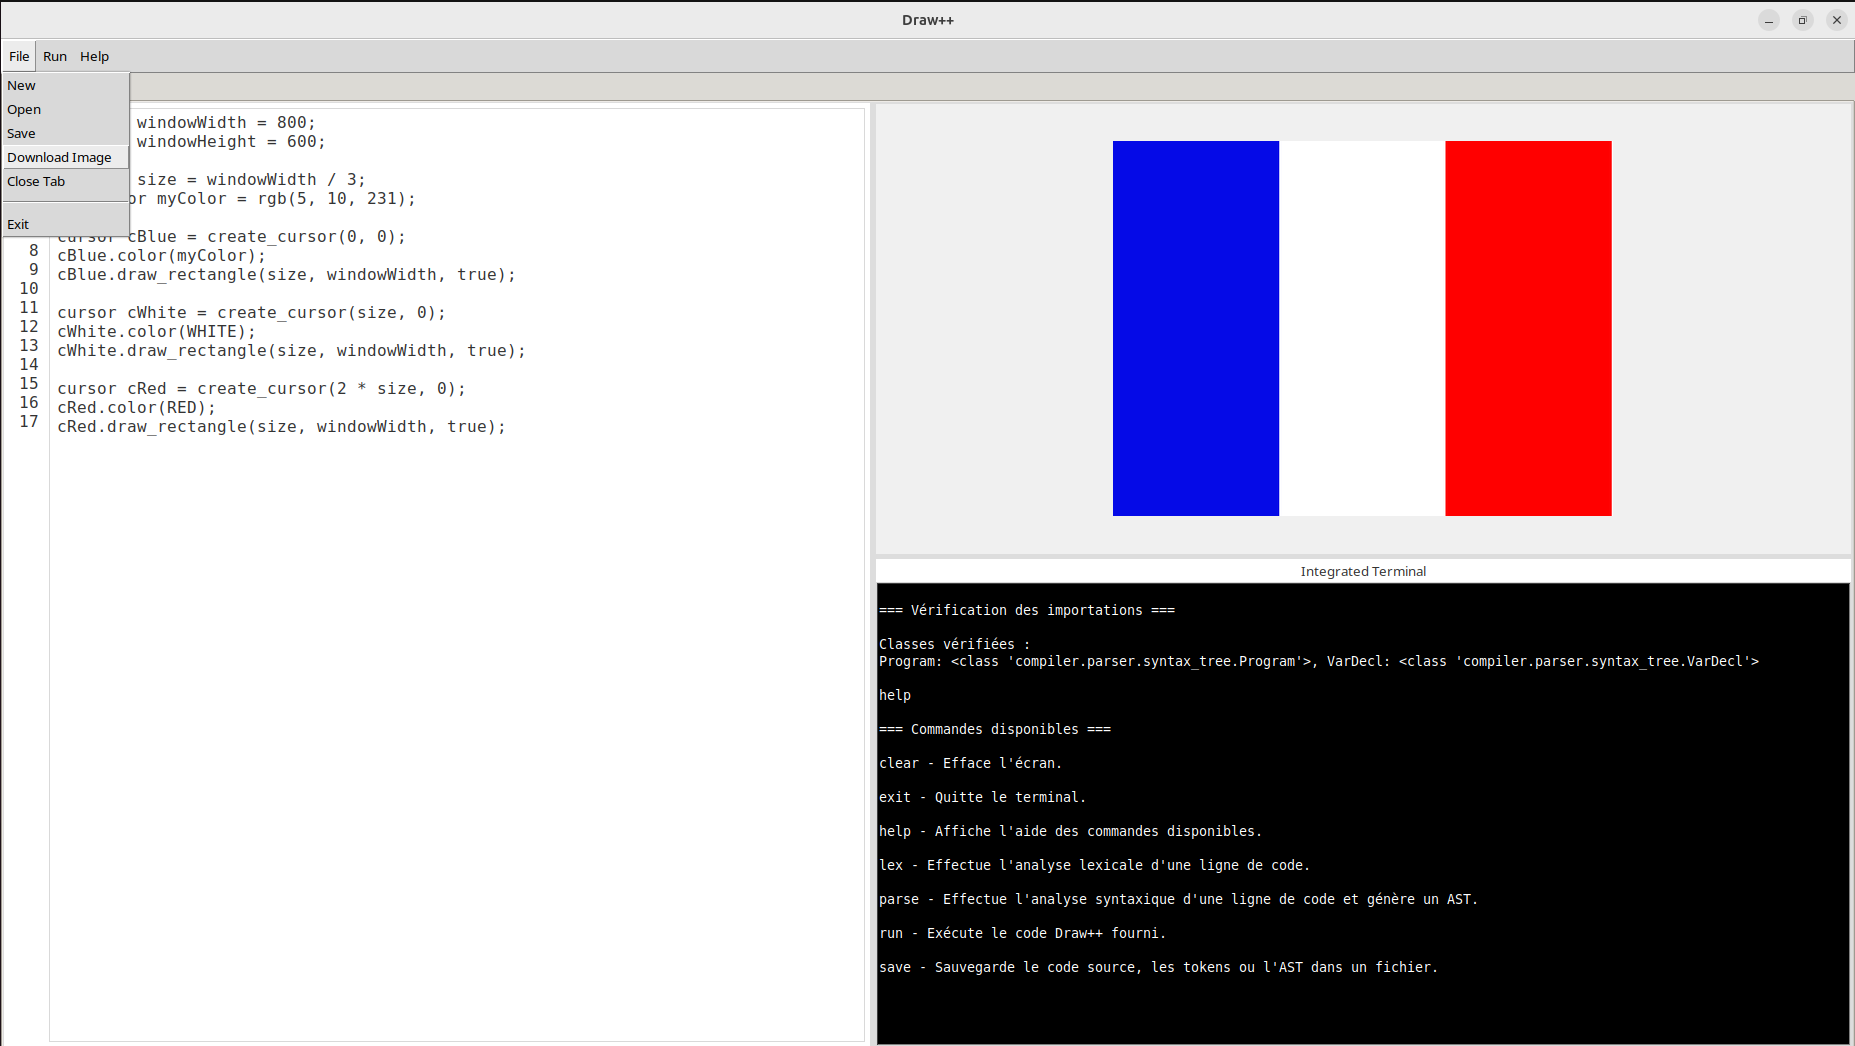
\includegraphics[width=0.9\linewidth]{image.png}
    \caption{Interface de Développement Intégré Draw++.}
    \label{fig:enter-label}
\end{figure}

\section{Composants principaux}

\subsection{Barre de menu}
La barre de menu en haut de l'interface offre plusieurs options essentielles :
\begin{itemize}
    \item \textbf{File} : Gestion des fichiers
    \begin{itemize}
        \item New : Créer un nouveau fichier
        \item Open : Ouvrir un fichier existant
        \item Save : Sauvegarder le fichier courant
        \item Download Image : Exporter le rendu graphique
        \item Close Tab : Fermer l'onglet actif
        \item Exit : Quitter l'application
    \end{itemize}
    \item \textbf{Run} : Exécution du code
    \item \textbf{Help} : Accès à l'aide
\end{itemize}

\subsection{Éditeur de code}
L'éditeur intègre plusieurs fonctionnalités avancées :
\begin{itemize}
    \item Numérotation automatique des lignes
    \item Coloration syntaxique pour le langage Draw++
    \item Mise en évidence des erreurs
    \item Support pour les commentaires (// et /* */)
\end{itemize}

\subsection{Zone de prévisualisation}
La zone de prévisualisation offre les caractéristiques suivantes :
\begin{itemize}
    \item Affichage du rendu graphique
    \item Mise à jour lors de l'exécution du code
    \item Zone redimensionnable
    \item Aperçu fidèle des dimensions spécifiées par \texttt{windowWidth} et \texttt{windowHeight}
\end{itemize}
\newpage
\subsection{Terminal intégré}
Le terminal propose plusieurs commandes essentielles :
\begin{lstlisting}[style=customStyle]
clear  - Efface l'ecran
exit   - Quitte le terminal
help   - Affiche l'aide des commandes disponibles
lex    - Effectue l'analyse lexicale d'une ligne de code
parse  - Effectue l'analyse syntaxique et genere l'AST
run    - Execute le code Draw++
save   - Sauvegarde le code source, les tokens ou l'AST
\end{lstlisting}


\section{Fonctionnalités d'analyse et débogage}

\subsection{Analyse lexicale}
Le terminal affiche les informations détaillées pour chaque token généré :
\begin{itemize}
    \item Type du token
    \item Valeur
    \item Numéro de ligne
    \item Position dans la ligne
\end{itemize}

Un exemple de sortie d'analyse lexicale :
\begin{figure}[H]
    \centering
    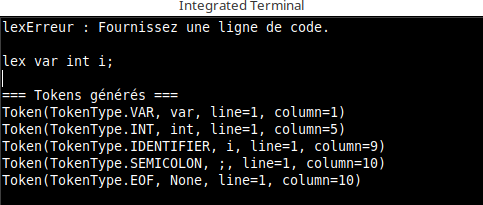
\includegraphics[width=0.7\linewidth]{terminal.png}
    \label{fig:enter-label}
\end{figure}

\subsection{Retours d'erreur}
L'IDE fournit des messages d'erreur détaillés pour différents types d'erreurs :
\begin{itemize}
    \item Erreurs de syntaxe
    \item Erreurs lexicales
    \item Erreurs sémantiques
    \item Problèmes de compilation
\end{itemize}

\subsection{Vérification en temps réel}
L'IDE effectue plusieurs vérifications pendant la saisie :
\begin{itemize}
    \item Validation des variables obligatoires (\texttt{windowWidth}, \texttt{windowHeight})
    \item Vérification de la syntaxe
    \item Détection des erreurs de type
    \item Validation des appels de méthodes sur les curseurs
\end{itemize}

\section{Bonnes pratiques d'utilisation}

\subsection{Initialisation du projet}
Pour démarrer un nouveau projet efficacement :
\begin{itemize}
    \item Toujours commencer par définir \texttt{windowWidth} et \texttt{windowHeight}
    \item Organiser le code avec des commentaires descriptifs
    \item Sauvegarder régulièrement le travail
\end{itemize}

\subsection{Débogage}
Pour un débogage efficace :
\begin{itemize}
    \item Utiliser la commande \texttt{lex} pour vérifier l'analyse lexicale
    \item Employer la commande \texttt{parse} pour valider la structure du code
    \item Consulter le terminal pour les messages d'erreur détaillés
\end{itemize}


\chapter{Exemples d'exécution}

Dans cette section, nous présentons plusieurs exemples d'exécution utilisant le langage Draw++. Chaque exemple inclut le rendu graphique généré et la sortie du terminal.

\section{Exemple 1 : Dessin d'un cercle}
\begin{figure}[H]
    \centering
    
\includegraphics[width=0.45\textwidth]{draw_circle.png}
    \caption{Rendu graphique du cercle.}
    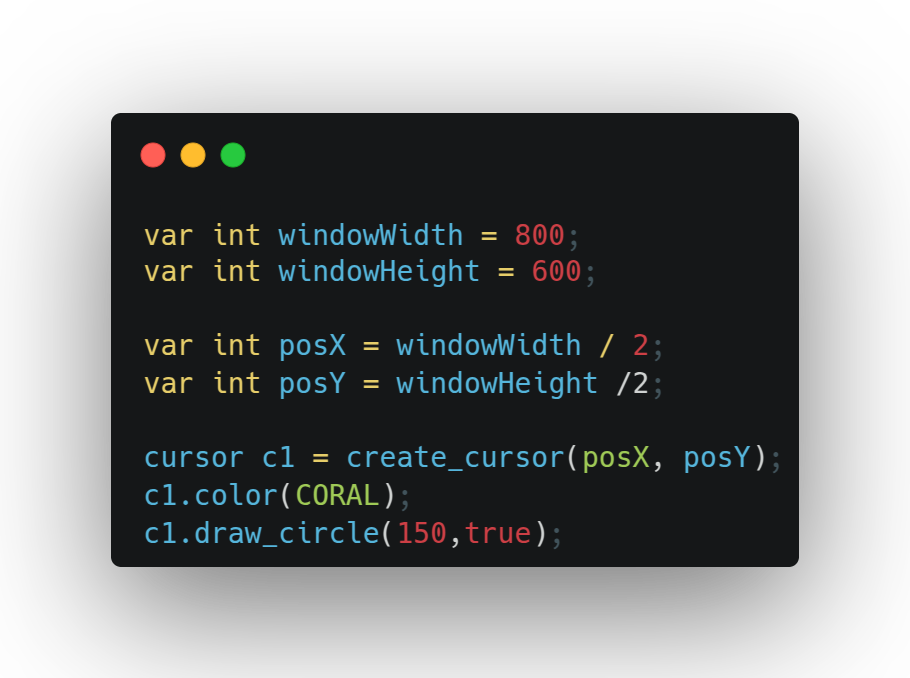
\includegraphics[width=0.9\textwidth]{draw_circle_dpp.png}
    \caption{Code DPP pour dessiner un cercle.}
\end{figure}

\section{Exemple 2 : Dessin d'un triangle}
\begin{figure}[H]
    \centering
    
\includegraphics[width=0.45\textwidth]{draw_triangle.png}
    \caption{Rendu graphique du triangle.}
    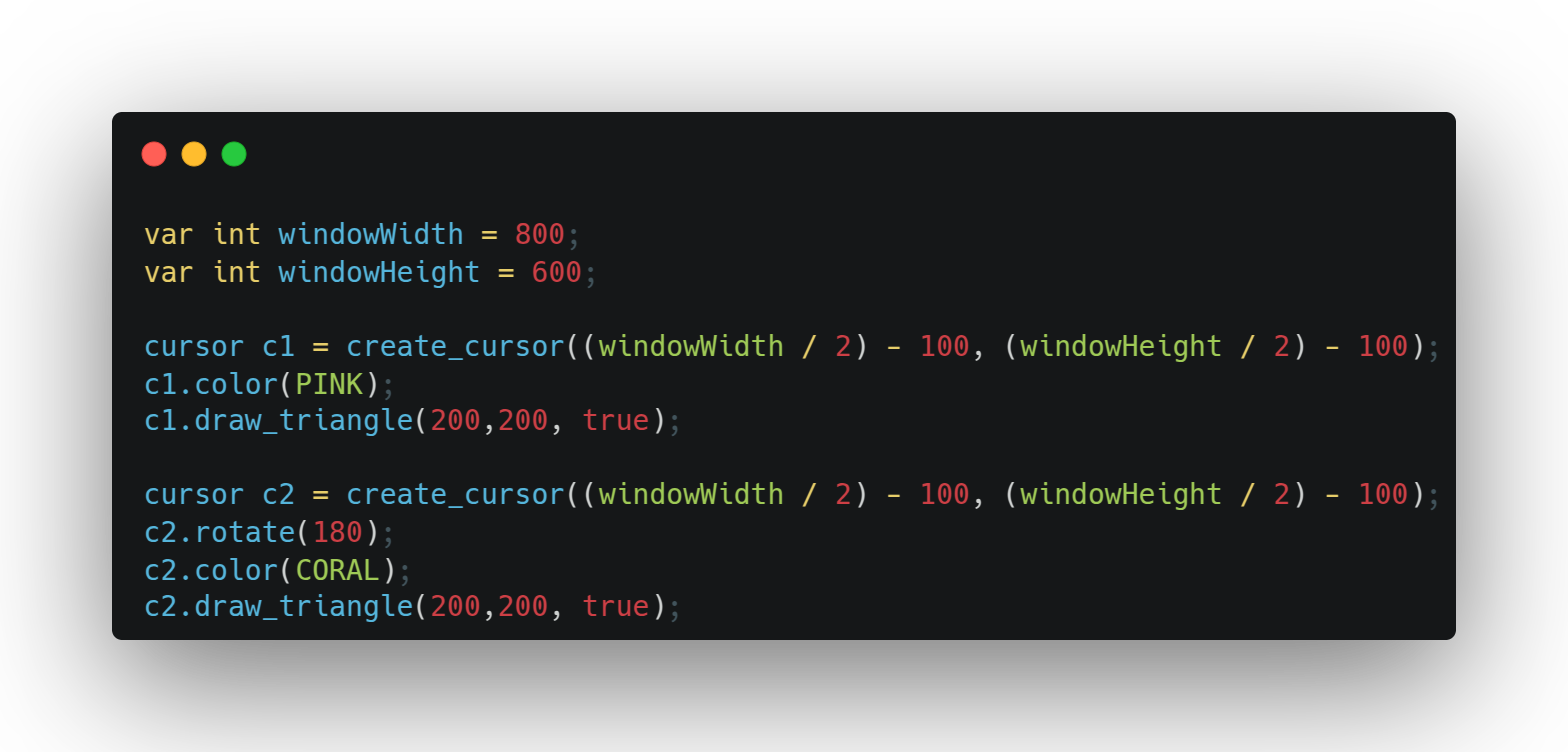
\includegraphics[width=0.9\textwidth]{draw_triangle_dpp.png}
    \caption{Code DPP pour dessiner un triangle.}
\end{figure}

\section{Exemple 3 : Dessin du drapeau de la France}
\begin{figure}[H]
    \centering
    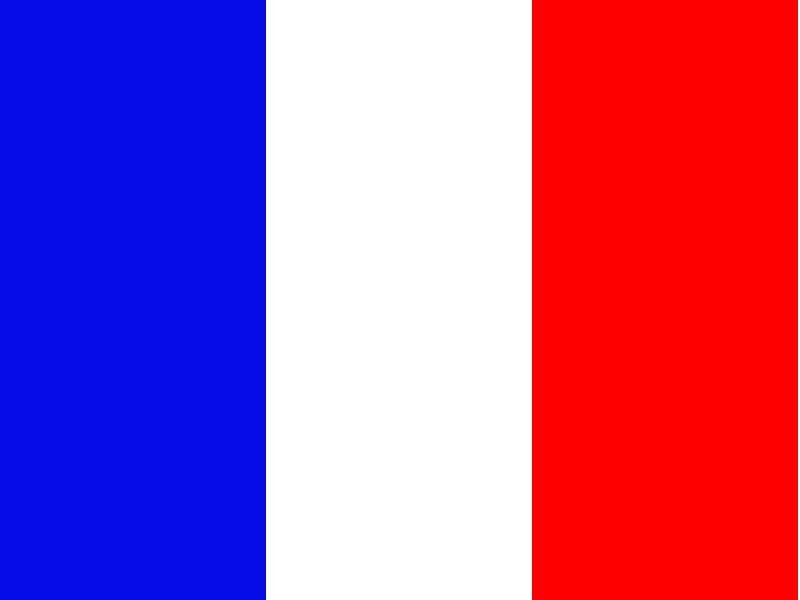
\includegraphics[width=0.45\textwidth]{france.png}
    \caption{Rendu graphique du drapeau de la France.}
    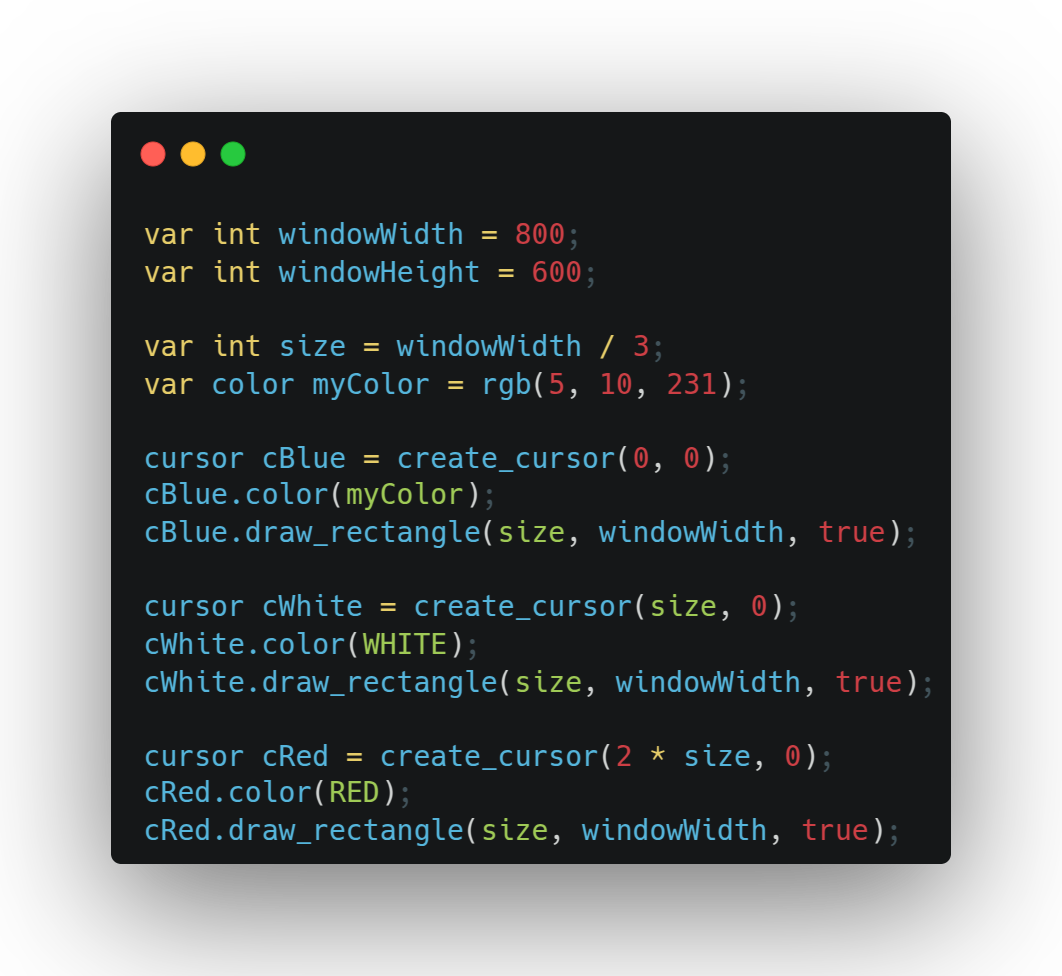
\includegraphics[width=0.8\textwidth]{france_dpp}
    \caption{Code DPP pour dessiner le drapeau de la France.}
\end{figure}

\section{Exemple 4 : Dessin d'une ligne}
\begin{figure}[H]
    \centering
    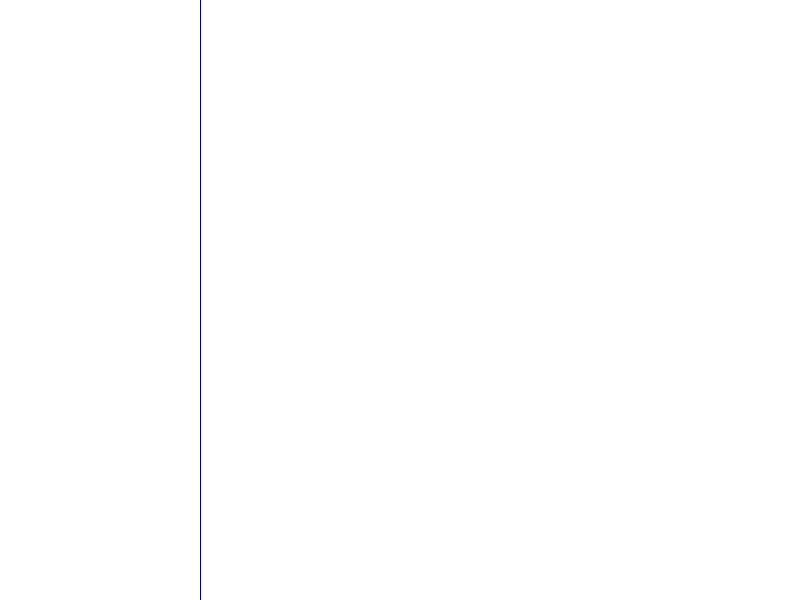
\includegraphics[width=0.45\textwidth]{draw_line.png}
    \caption{Rendu graphique de la ligne.}
    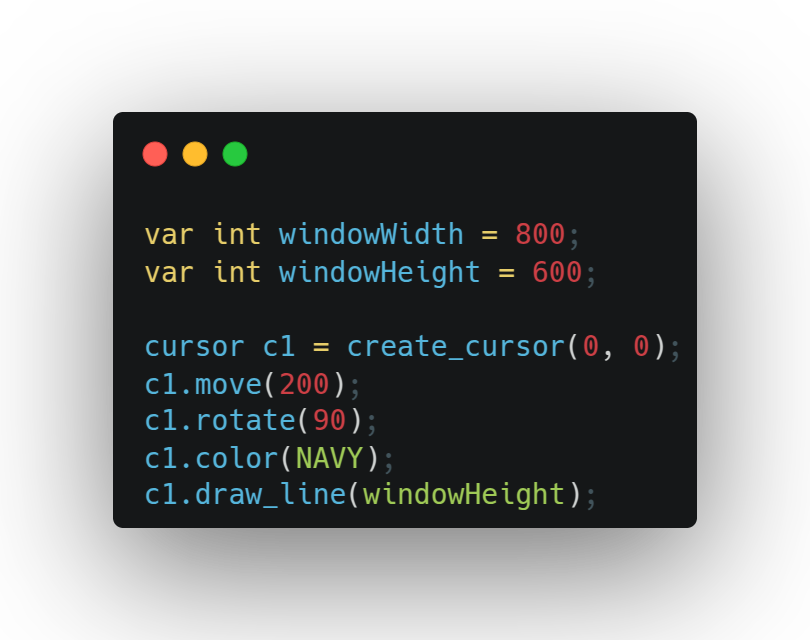
\includegraphics[width=0.8\textwidth]{draw_line_dpp.png}
    \caption{Code DPP pour dessiner une ligne.}
\end{figure}

\section{Exemple 5 : Dessin d'un rectangle}
\begin{figure}[H]
    \centering
    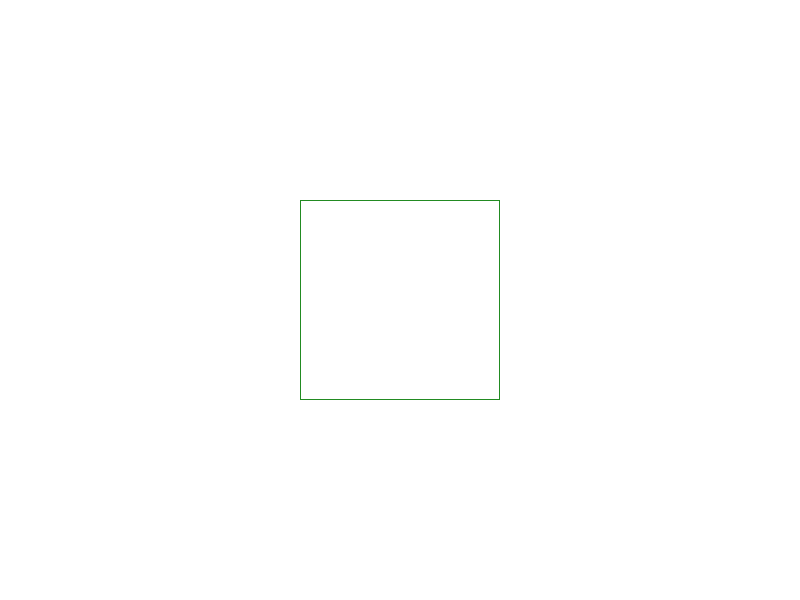
\includegraphics[width=0.7\textwidth]{draw_rectangle.png}
    \caption{Rendu graphique du rectangle.}
    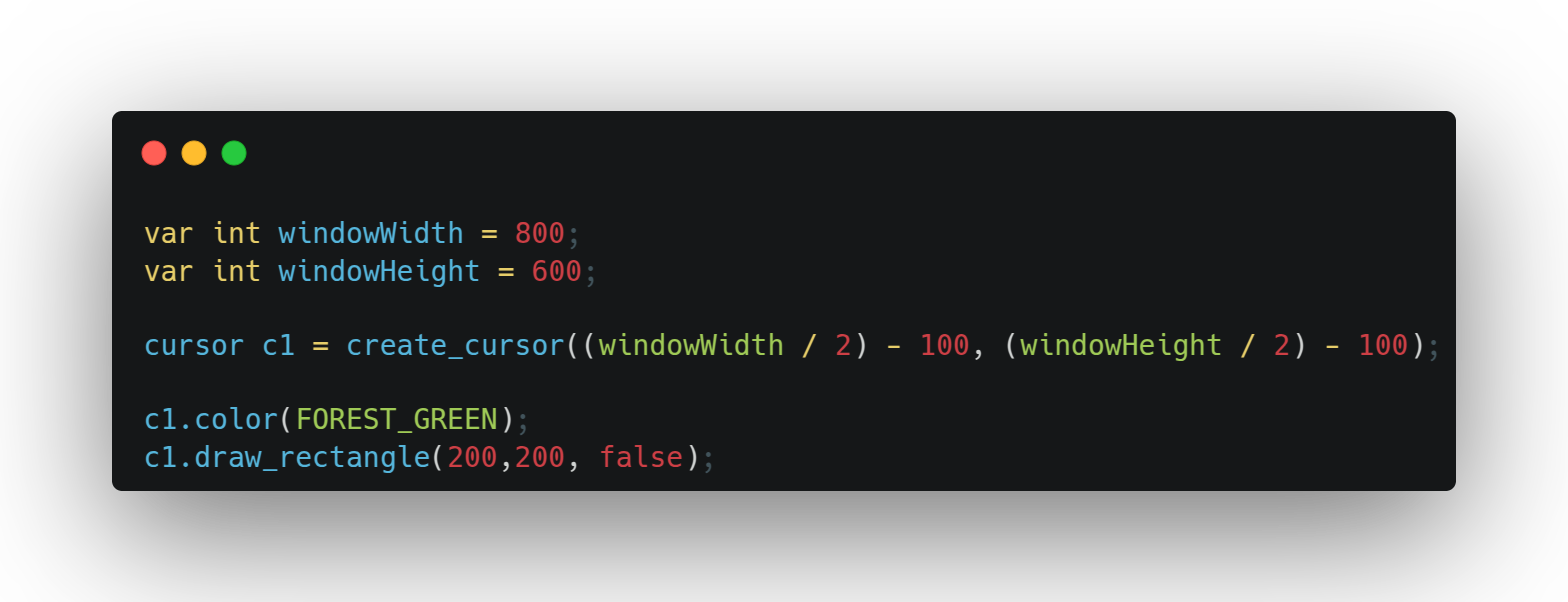
\includegraphics[width=1\textwidth]{draw_rectangle_dpp.png}
    \caption{Code DPP pour dessiner un rectangle.}
\end{figure}

\section{Exemple 6 : Dessin d'une ellipse}
\begin{figure}[H]
    \centering
    
\includegraphics[width=0.45\textwidth]{draw_ellipse.png}
    \caption{Rendu graphique de l'ellipse.}
    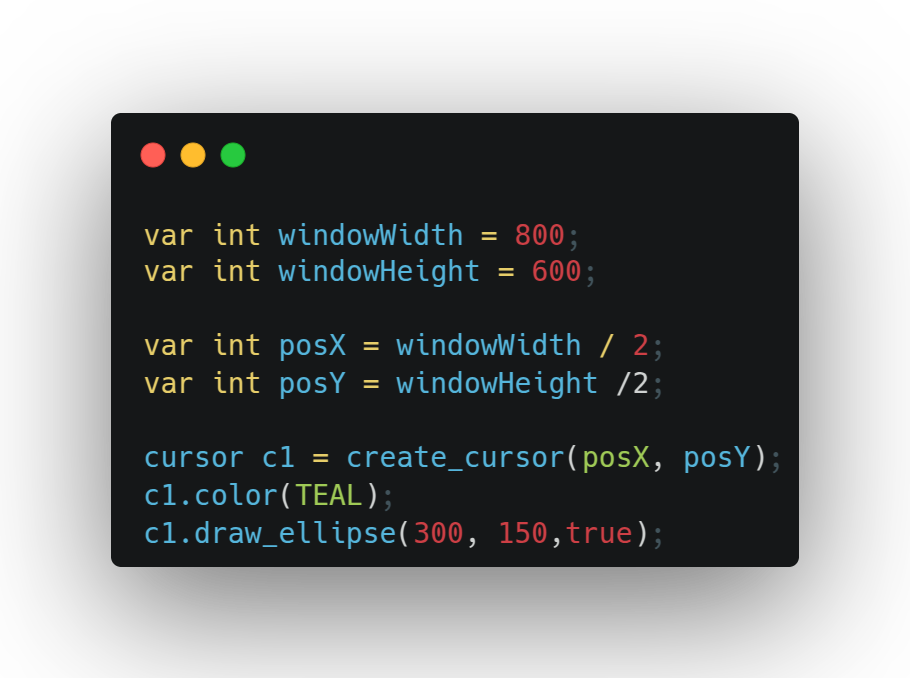
\includegraphics[width=0.8\textwidth]{draw_ellipse_dpp.png}
    \caption{Code DPP pour dessiner une ellipse.}
\end{figure}

\newpage

\section{Sortie du terminal}
\begin{figure}[H]
    \centering
    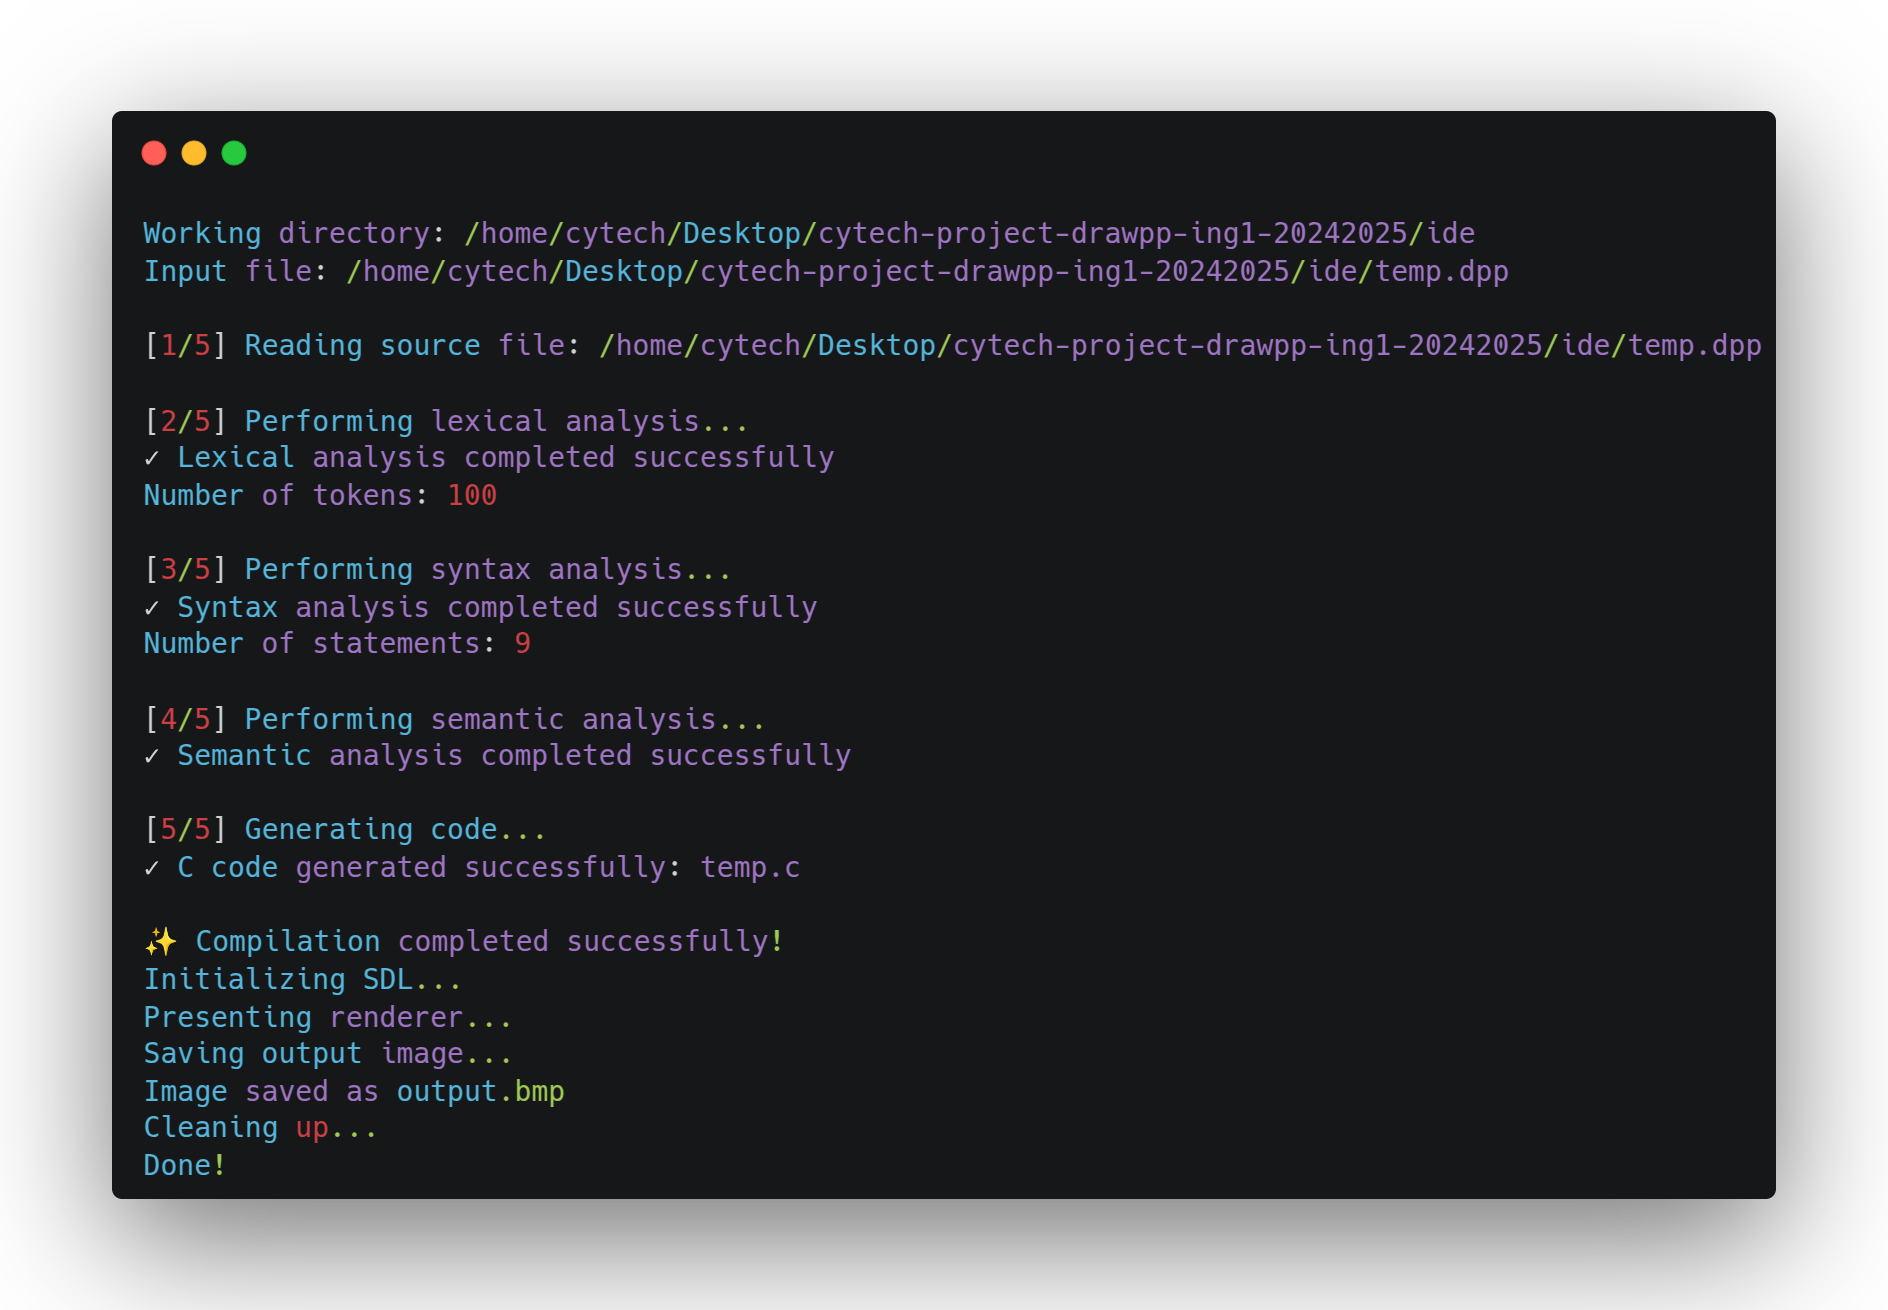
\includegraphics[width=1\textwidth]{terminal_output_after_run.png}
\end{figure}

 \chapter{Conclusion}

Le projet Draw++ a permis la conception d'un langage graphique minimaliste, couplé à un traducteur robuste, capable de transformer des instructions simples en formes visuelles. Le traducteur, conçu avec une attention particulière à la gestion des erreurs et à l’analyse syntaxique, garantit une exécution fluide et précise du code. La structure du langage, combinée à des outils de manipulation des formes, offre une plateforme puissante pour explorer l'interaction entre programmation et visualisation graphique.





\end{document}